\documentclass{article}
\usepackage{geometry}
\usepackage{listings}
\usepackage{color}
\usepackage{hyperref}
\usepackage{graphicx}
\usepackage{float}
\usepackage{sectsty}
\usepackage{enumitem}

\definecolor{codebackground}{rgb}{0.99,0.99,0.97}
\definecolor{mygray}{rgb}{0.5,0.5,0.5}

\lstset{
    basicstyle=\ttfamily,
    backgroundcolor=\color{white},
    keywordstyle=\color{blue},
    commentstyle=\color{mygray},
    showstringspaces=false,
    numbers=left,
    numberstyle=\tiny,
    numbersep=5pt,
    breaklines=true,
    frame=single,
    breakatwhitespace=false,
}

\geometry{a4paper, margin=0.75in}

\title{\textbf{CS3510 - Operating System}\\Assignment 1}
\author{\textbf{Soham Rajesh Pawar}\\CS22BTECH11055}
\date{November 27, 2023}

\begin{document}
\maketitle

\section{Introduction}
{\large In the realm of operating systems, the efficient utilization of resources is paramount. This report delves into the implementation of a program in C that explores the world of tetrahedral numbers, leveraging parallel processing to enhance performance. The assignment involves breaking down the task among multiple child processes to compute tetrahedral numbers within a given range.
}
\section{Coding Approach}
{\large
The program, implemented in C, takes a novel approach to find tetrahedral numbers efficiently. Utilizing shared memory for communication between processes enhances parallelism, allowing for a more streamlined computation process. The assignment was approached systematically, dividing the workload among multiple child processes to exploit the capabilities of modern multi-core systems.
}
\subsection{Steps}
\begin{enumerate}
  \item{Read \texttt{N} and \texttt{K} from the input file to define the computation range and the number of child processes.}
  \item{Allocate shared memory segments to facilitate communication between the main process and child processes.}
  \item{Create \texttt{K} child processes, each assigned a unique range of numbers to check for tetrahedrality.}
  \item{Distribute the workload based on the process ID, ensuring each process examines a distinct subset of numbers.}
  \item{For each number in its allotted set, a process records its tetrahedrality status in its respective log file. Additionally, on identifying a tetrahedral number, the process stores the number in its shared memory.}
  \item{The main process waits for the completion of all child processes.}
  \item{Access the shared memory of each process, recording the identified tetrahedral numbers (if any) in the main log file.}
\end{enumerate}

\section{Verification}
{\large
The verification process involves rigorous checks to validate the correctness of the program's output. Special attention is given to handling edge cases and potential pitfalls that might affect the accuracy of the results.

\section{Conclusion}
{\large
In conclusion, the implemented program showcases the efficiency of parallel processing in tackling computational tasks. The analysis of execution times and the impact of varying parameters provides valuable insights into the scalability and performance of the solution.

\section{Graphs}
\subsection{Maintaining \texttt{K} at 8\\Time vs Size($2^{3N}$) :}
\begin{figure}[H]
  \centering
  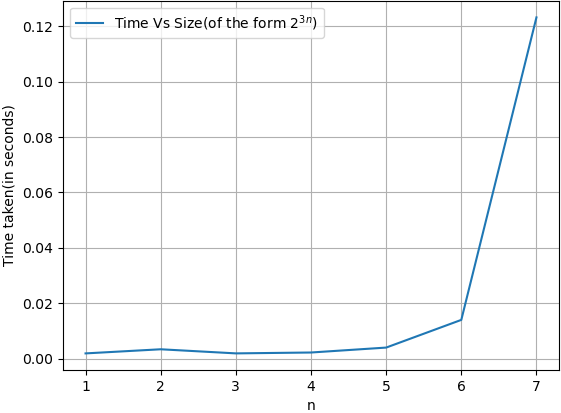
\includegraphics[width=0.6\linewidth]{1.png}
  \caption{Relationship between execution time and input size with \texttt{K} set to 8.}
  \label{fig:graph1}
\end{figure}

\subsection{Maintaining Size at 10,00,000\\Time vs Number of Processes (\texttt{K}) :}
\begin{figure}[H]
  \centering
  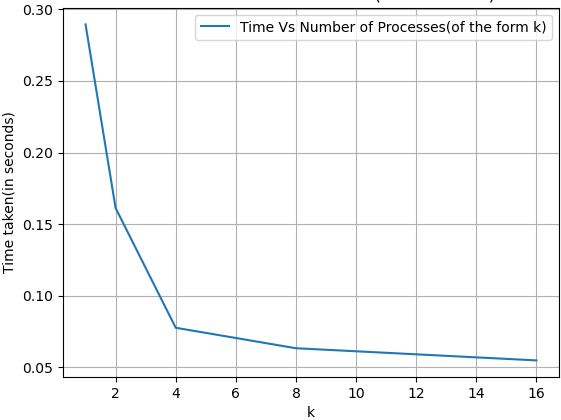
\includegraphics[width=0.6\linewidth]{2.png}
  \caption{Impact of varying the number of processes (\texttt{K}) on execution time with a fixed input size.}
  \label{fig:graph2}
\end{figure}
\end{document}

